\documentclass[letterpaper, 12pt]{article}
\usepackage[utf8]{inputenc}
\usepackage[margin=1in]{geometry}
\usepackage{amsmath}
\usepackage[affil-it]{authblk}
\usepackage{verbatim}
\usepackage{todonotes}
\usepackage{setspace}
\usepackage{graphicx}
\usepackage{float}
\usepackage{wrapfig}
\usepackage{hyperref}
\usepackage{bbold}
\usepackage{url}
\usepackage{fancyhdr}

\fancypagestyle{headerstyle}
{
   \fancyhf{}
	\fancyfoot[C]{\textbf{CONFIDENTIAL MATERIAL: DO NOT COPY OR DISTRIBUTE WITHOUT SPONSOR’S PERMISSION.}}
	\renewcommand{\headrulewidth}{0pt}
	\renewcommand{\footrulewidth}{0pt}
}

\fancyhf{}
\fancyfoot[C]{\thepage}
\renewcommand{\headrulewidth}{0pt}
\renewcommand{\footrulewidth}{0pt}

\pagestyle{fancy}

\makeatletter
%\let\ps@plain\ps@fancy 
\let\ps@plain\ps@headerstyle 
\makeatother


\begin{document}

\title{\vspace{30mm}An Improved Approach to Model Epistatic Interactions Among Multiple Genetic Variants Using Pleiotropy}
\author{\vspace{20mm}Tian-Shun Allan Jiang}

\affil{%\vspace{8mm}
Stanford University,\\NC School of Science and Mathematics}

\author{Gregory Carter}
\affil{%\vspace{8mm}
The Jackson Laboratory}

\date{The Jackson Lab Summer Student Program\\
\vspace{5mm} \today}

\singlespace
\maketitle

\listoftodos

\newpage

\doublespace

\section*{Introduction}

One area of focus in systems biology is the use of quantitative and statistical genetics to understand how genetic variants combine to influence complex traits. Advances in high-density genotyping and multidimensional phenotyping can produce highly detailed views of biological systems for this purpose. However, extracting meaningful biological models for human health and disease from these large datasets will require the creation of new analytical methods and software.

One promising approach to use this data is in the systematic study of genetic interactions as a way to map genetic networks \cite{boone2007}. These networks can then be used to infer functional relationships in molecular biology such as activation, repression, and pathway ordering \cite{avery1992ordering}. Previous work by Carter et al.\ \cite{carter2013fly,carter2012yeast} created mathematical models to infer genetic networks from epistatic interactions using various fly and yeast crosses exhibiting partial pleiotropy. These models were then used on some well-studied biological systems, such as the reproductive pathway in yeast \cite{carter2012yeast} to confirm wet-lab results found in literature.

However, interactions detected by existing models only analyse two genetic variants at a time and thus may not provide a complete model of epistasis. In this paper, we create a more complete model of epistasis by extending the previous model to incorporate multiple genetic variants at a time, which can help uncover novel interactions and detect indirect variant-to-variant influences. 

\todo[inline]{Summarize what you've done with little cross dataset, like in Carter 2013}

\begin{comment}
What are the ideas?
\begin{enumerate}
\item Advances in genomic/phenotypic technologies allow us to gather a lot of data which need new methods of studying \cite{tyler2013cape}
\item We want to map genetic networks using interaction analysis on a \textbf{genome-scale}. Has been done in yeast worm and fly. \cite{carter2013fly}
\item New mouse populations allow us to conduct interaction analysis in mammalian models for ``activation, repression, and pathway ordering" \cite{carter2012yeast}
\end{enumerate}
\end{comment}

\section*{Methods}
\subsection*{Data Source}
Data were obtained from a study of \todo{write about the data...}

\subsection*{Genetic Interaction Model}
Since our model extends upon previous data analysis techniques by Carter et al.\ which are described at length in previous publications \cite{carter2013fly, carter2012yeast}, we summarize the known analysis procedures here, and cover novel techniques and ideas in higher detail. All of the previously known analysis techniques were performed using the software package \texttt{R/cape} \cite{tyler2013cape}.

\subsubsection*{1. Singular Value Decomposition}
First, we performed singular value decomposition (SVD) on our mean-centered, standard-deviation-normalized phenotype data to maximize orthogonality. This allows us to fully exploit the complementary phenotype data by reducing linear dependence. Then we chose the first five left singular vectors for analysis. For convenience, we hereafter refer to these left singular vectors as ``eigentraits".
\todo[size=\tiny]{In our data, these eigentraits captured x\% of the variance.}

\missingfigure{Show plotSVD that has percent variance plots}

\subsubsection*{2. Singlescan to find covariates}

Then, we performed a linear regression for each of the 100 genes to identify strong-effect genetic variants to be treated as additive covariates in subsequent pairwise regressions. For each locus we performed the regression: 

\begin{equation} \label{eq:singlescan}
U^{j}_{i} = \beta^{j}_{0} + \beta^{j}_{1}x_i + \epsilon^{j}_{i}
\end{equation}

where $i$ is looped over all individuals in the population, $j$ is looped over all eigentraits, $U^{j}_{i}$ is the value of eigentrait $j$ for individual $i$, $\beta^{j}$ is the effect of the effect of the locus on eigentrait $j$, and $\epsilon^{j}_{i}$ is the residual error. In our data, each of the $x_{i}$ genotype values were either $0, 1$ or $2$, corresponding to the AA, AB, and BB genotypes. Genotypes are encoded this way by the additive assumption of variants on phenotypes. Then, strong-effect knockdowns are identified as significant $\beta^{j}_{1}$ coefficients, which are then included as covariates for the associated phenotype. 
%Then, we use those covariates and perform a ``pairscan" regression, which models all possible variant pairs with main effects and an interaction term. For example, in a pairscan using variants 1 and 2 we get:

Here is where our analysis extends upon methodology by Carter et al.\ \cite{carter2013fly,carter2012yeast}. Previous methodology conducted a ``pairscan", shown below for sample variants 1 and 2.

\begin{equation}
U^{j}_{i} = \beta^{j}_{0} + \underbrace{\sum_{c}x_{c,i}\beta_{c}^j}_{\text{Covariates}} +  \underbrace{\beta^{j}_{1}x_{1i} + \beta^{j}_{2}x_{2i}}_{\text{Main Effects}} + \underbrace{\beta^{j}_{2}x_{1i}x_{2i}}_{\text{Interaction}} + \epsilon^{j}_{i}
\end{equation}

The variables are the same as those in Equation \ref{eq:singlescan}, with the additional interaction term $\beta_{12}^j$ and the addition of strong-effect knockdowns as covariates. This interaction term can be reparameterized into variant-to-variant influences, but is limited by the fact that it can only model interactions between two variants at a time. 

\subsubsection*{3. Extending the model to $n$ variants}

Here, we extend the model to the analysis of $n$ variants as follows:

\begin{equation}
U^{j}_{i} = \beta^{j}_{0} + \underbrace{\sum_{c}x_{c,i}\beta_{c}^j}_{\text{Covariates}} +  \underbrace{\sum_{a=1}^{n}\beta^{j}_{1}x_{ai}}_{\text{Main Effects}} + \underbrace{\sum_{a,b}\beta^{j}_{ab}x_{ai}x_{bi}}_{\text{all pairs }a,b} + \underbrace{\sum_{a,b,c}\beta^{j}_{abc}x_{ai}x_{bi}x_{bi}}_{\text{all triples }a,b,c} + \ldots + \epsilon^{j}_{i}
\end{equation}

This regression models combined variant interaction effects among $n$ variants, as it includes terms for any combination of variants under analysis. For example, the $\beta_{abc}^j$ coefficient represents the strength of the interaction among variants $a,b$ and $c$ in explaining the variance of eigentrait $j$.

To resolve these combined interaction coefficients into variant-to-variant influences, we first reparameterize the interaction coefficients in terms of variables $\delta_{ab}$ and $\delta_{ba}$ for all combinations of variants $a$ and $b$ from the $n$ variants of interest.

The value of $\delta_{ab}$ represents the change in genotype value in variant $b$ when the perturbation in variant $a$ is present (i.e. when variant $a$ is not homozygous for the reference strain). This way, genetic interactions are quantified as the phenotype-relevant activity of each variant is altered according to the value of $\delta$.

\section*{Results}

\section*{Discussion}

\newpage

\bibliographystyle{plain}
\bibliography{references}

\end{document}

%======================================================
%======================================================
%================Document ends here!=========================
%======================================================
%================Notes being below!==========================
%======================================================
%======================================================

Document is online:
https://docs.google.com/document/d/1Ow97N7w9jhJ7RWqQ-gROuoLHtffS94VSSVpHRCWtpOI/edit?usp=sharing
WYSIWYG life oops


This study aims to create a mathematical model to more accurately detect epistasis (gene-gene interactions) among multiple genetic variants using the existence of partial pleiotropy (when one gene affects multiple phenotypes). Previous methods to detect epistatic interactions have been defined \cite{carter2012yeast}, but may fail to produce the most complete model of the genetic network. This study aims to extend previous models to more accurately model epistatic interactions among multiple loci and to create an open-source software package in \texttt{R} to allow other researchers to replicate the same data analysis.

%\subsubsection*{Background}
One area of focus in systems biology is the use of quantitative and statistical genetics to understand how genetic variants combine to influence complex traits. Recent advances in high-density genotyping and multidimensional phenotyping can produce highly detailed views of biological systems for this purpose. However, extracting meaningful models for health and disease from these large datasets will require the creation of new analytical methods and software. 

One potentially promising approach to use this data is in the study of genetic interactions. Previous work by Carter et al.\ \cite{carter2013fly,carter2012yeast} created mathematical models to detect epistatic interactions from various fly and yeast crosses exhibiting partial pleiotropy, and Tyler et al.\ \cite{tyler2013cape} implemented the methodology by publishing an open-source \texttt{R} package called \texttt{cape} to conduct the statistical analysis. These models were then used on some well-studied biological systems, such as the reproductive pathway in yeast \cite{carter2012yeast}, to confirm wet-lab results found in literature. However, due to the method's usage of pair-wise analysis of genetic variants, it also detected some additional novel genetic interactions which could be false positives. Thus, our goal in improving the model is to limit the number of false positives in the genetic network.

%\subsubsection*{Experimental Approach:}
We hypothesize that analyzing interactions between multiple ($n \geq 3$) variants at once (instead of a pair-wise analysis) will aid in minimizing detection of false positives while maintaining the statistical power to pick up true interactions. In order to test this hypothesis, the following steps will be taken:
\begin{enumerate}
\item Create candidate mathematical models for the analysis of $n$ genetic variants
\item Evaluate the models based on performance on fabricated data
\item Evaluate model robustness by adding varying levels of noise to the fabricated data
\end{enumerate}
This methodology should help to create a more accurate and robust model for the detection of variant-to-variant interactions while avoiding false positive interactions. The resulting genetic network created by the analysis can help to translate statistical epistasis in a large dataset into a precise and testable hypothesis.


http://www.math.uni-leipzig.de/~hellmund/LaTeX/pgf-tut.pdf
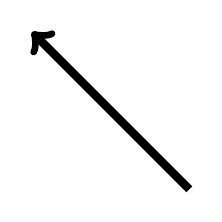
\begin{tikzpicture}[scale=1]
\draw [line width=3pt,->] (2,0) -- (0,2);
\end{tikzpicture}

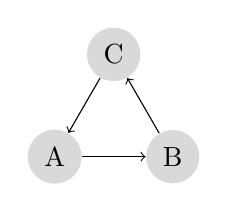
\begin{tikzpicture}[scale=1, transform shape] %transform shape scales node sizes as well
\tikzstyle{every node} = [circle, fill=gray!30]
\node (a) at (0, 0) {A};
\node (b) at +(0: 1.5) {B}; %+ is polar coordinates!
\node (c) at +(60: 1.5) {C};
\foreach \from/\to in {a/b, b/c, c/a}
\draw [->] (\from) -- (\to);
\end{tikzpicture}

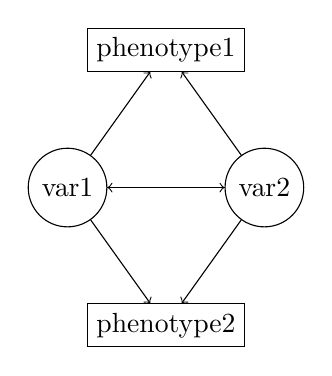
\begin{tikzpicture}[scale=1, transform shape] %transform shape scales node sizes as well
\node[draw, shape=circle]       (a) at (0, 0) {var1};
\node[draw, shape=circle]       (b) at (2.5, 0) {var2};
\node[draw, shape=rectangle] (c) at (2.5/2, 1.75) {phenotype1};
\node[draw, shape=rectangle] (d) at (2.5/2, -1.75) {phenotype2};
\foreach \from/\to in {a/b, b/a, b/c, a/c, b/d, a/d}
\draw [->] (\from) -- (\to);
\end{tikzpicture}
